\documentclass[oneside,reqno]{amsart}
\usepackage{amsthm}
\usepackage{dsfont}
\setlength{\textwidth}{\paperwidth}\addtolength{\textwidth}{-2in}\calclayout
\usepackage[utf8]{inputenc}
\usepackage{tikz}
\usepackage{minted}
\newminted{python3}{frame=lines}
\usepackage{booktabs}
\usepackage{enumitem}
\setlist[enumerate]{label={(\roman*)}}

\DeclareMathOperator{\E}{E}
\DeclareMathOperator{\var}{var}
\DeclareMathOperator{\cov}{cov}
\DeclareMathOperator{\corr}{corr}
\newcommand{\eps}{\varepsilon}
\newcommand{\ups}{\upsilon}

\theoremstyle{definition}
\newtheorem{prob}{Problem}
\renewcommand*{\proofname}{Solution}

\title{ECON 706: Problem Set 4}
\author{Daniel Pfeffer}
%------------------------------------------------------------------------------
\begin{document}
\maketitle

\begin{prob}\label{prob1}
\textbf{Estimating a Trend-Stationary Model}
\end{prob}

\begin{enumerate}
\item
Download quarterly U.S. real GDP from the FRED database maintained by the Federal Reserve Bank of St. Louis for 1985:Q1 to 2019:Q4.

\begin{proof}
Query real GDP data for 1985:Q1 to 2019:Q4 from the FRED. 
\begin{python3code}
import numpy as np
import pandas as pd
import pandas_datareader.data as web
import datetime

# 1985:Q1 to 2019:Q4
start = datetime.datetime(1985, 1, 1)
end = datetime.datetime(2019, 12, 31)

# Quarterly U.S. real GDP from the FRED
ts = web.DataReader('GDPC1', 'fred', start, end)
\end{python3code}
\end{proof}

\item
What do we mean by quarterly GDP? Goods and services produced within the quarter, or the goods and services that would be produced in the calendar year if the output during the quarter prevails over 12 months?

\begin{proof}
According to the FRED, the GDPC1 series is measured in ``Billions of Chained 2009 Dollars, Seasonally Adjusted Annual Rate''. So quarterly GDP refers to the goods and services that would be produced in the calendar year if the output during the quarter prevails over 12 months.
\end{proof}


\item
Now consider the following model:
\begin{equation}\label{eq:1}
	y_t = \gamma_1  + \gamma_2 t + \tilde y_t, 
	\qquad 
	\tilde y_t = \rho  \tilde y_{t-1} + \eta_t,
	\qquad 
	\eta_t \sim \text{iid N} (0, \sigma_\eta^2),
\end{equation}
where $y_t := \log \text{GDP}_t$. Rewrite the model as 
\begin{equation}\label{eq:2}
	y_t = \beta_1 + \beta_2 t + \beta_3 y_{t-1} + \eps_t,
	\qquad 
	\eps_t \sim \text{iid N}(0, \sigma_\eps^2).
\end{equation}
What is the relationship between $(\gamma_1, \gamma_2, \rho, \sigma_\eta^2)$ and $(\beta_1, \beta_2, \beta_3, \sigma_\eps^2)$?

\begin{proof}
Using lag operators, we can write
\[
	(1-\rho L)y_t = \eta_t
\]
and express \eqref{eq:1} as  
\[
	y_t = \gamma_1 + \gamma_2  t + (1-\rho L)^{-1} \eta_t,  
\]
provided $(1-\rho L)^{-1}$ exists. Then applying the quasi-difference operator $\Delta^\rho := (1-\rho L)$ to both sides gives 
\begin{align*}
	\Delta^\rho y_t &= (1-\rho L)(\gamma_1 + \gamma_2 t + (1-\rho L)^{-1} \eta_t)\\
	&= \gamma_1+ \gamma_2 t - \rho \gamma_1 - \rho \gamma_2(t-1) + \eta_t \\
	&=(1-\rho)\gamma_1 + \rho \gamma_2 + (1-\rho)\gamma_2 t + \eta_t
\end{align*}
or
\[
	y_t = (1-\rho)\gamma_1 + \rho \gamma_2 + (1-\rho)\gamma_2 t+ \rho y_{t-1} + \eta_t.
\]
Hence $(\beta_1, \beta_2, \beta_3, \sigma_\eps^2) = ( (1- \rho) \gamma_1 + \rho \gamma_2, (1-\rho)\gamma_2, \rho, \sigma_\eta^2)$.
\end{proof}

\item
Estimate \eqref{eq:2} by OLS. What is your estimate of the average growth rate of output (be precise about the units of measurement)? What is the estimated autocorrelation of the fluctuations around the deterministic trend?

\begin{proof}
The following code estimates \eqref{eq:2} by OLS.
\begin{python3code}
import statsmodels.api as sm

# Add constant
ts = sm.add_constant(ts)

# Add trend variable 
ts['trend'] = ts.const.cumsum()

# Log transformation
ts['y'] = np.log(ts['GDPC1'])

# Add lag term
ts['y_lag1'] = ts['y'].shift()

# Drop first observation
ts = ts[1:]

# Fit model by OLS
mod = sm.OLS(ts['y'], ts[['const', 'trend', 'y_lag1']])
res = mod.fit()
\end{python3code}

Since $\gamma_2$ in \eqref{eq:1} can be interpreted as the quarterly growth rate, an estimate of average quarterly growth rate can be obtained through the relation in (i), which implies $\gamma_2 = \beta_2/(1- \beta_3)$. Using the the OLS regression results in Table \ref{ols-res}, the estimated average quarterly growth rate of approximately 0.42\% or 1.5\% per year, a poor estimate, since the actual average annual growth rate is roughly 2-3\%. 
\par
To obtain the estimated autocorrelation of the fluctuations around the deterministic trend, since $\beta_3 = \rho$, we obtain an estimate of approximately $0.988$, which indicates that the estimated process is highly persistent. This evidence suggests that this trend-stationary model is not a good choice and that the real GDP process perhaps contains a stochastic tend component. 

\begin{table}[!h]
\caption{OLS regression results of Equation \eqref{eq:2}.}
\begin{center}
\begin{tabular}{lc}
\hline
          &    $\log \text{GDP}_t$      \\
\midrule
const     & 0.117     \\
          & (0.105)   \\
trend     & 0.000     \\
          & (0.000)   \\
$\log \text{GDP}_{t-1}$    & 0.988***  \\
          & (0.012)   \\
\hline
%Standard errors in parentheses. \\
* $p<.1$, ** $p<.05$, \\
*** $p<.01$
\end{tabular}
\end{center}
\label{ols-res}
\end{table}
\end{proof}

\item
Use your OLS estimates of $\beta$ and iterate \eqref{eq:2} forward starting from $y_1$ and setting the error terms to zero. Plot the resulting trajectory and setting the error terms to zero. Plot the resulting trajectory and compare it to plots of $\tilde y_t = \hat \beta_1 + \hat \beta_2 t$ and $\hat y_t = \hat \beta_1 + \hat \beta_2 t + \hat\beta_3 y_{t-1}$, where now you use the observed value $y_{t-1}$. Discuss. 

\begin{proof}
The following code generates Figure \ref{q1-fig}.

\begin{python3code}
# Generate trajectory
beta1 = res.params.values[0]
beta2 = res.params.values[1]
beta3 = res.params.values[2]
y = [ts['y'][0]]
for t in range(1, len(ts)):
    y.append(beta1 + beta2*ts['trend'][t] + beta3*y[t-1])

# Generate y_tilde     
y_tilde =  beta1 + beta2*ts['trend']

# Plot results
import matplotlib.pyplot as plt

fig, [ax1, ax2] = plt.subplots(1, 2, figsize=(12,4))

ax1.plot(mod.data.orig_endog, label='$y_t$')
ax1.plot(res.fittedvalues, label='$\hat y_t$')
ax1.plot(ts.index, y, label='Trajectory')
ax1.legend()

ax2.plot(ts.index, y)
ax2.plot(res.fittedvalues)
ax2.plot(y_tilde, color='r', label='$\tilde y_t$')
ax2.legend()

plt.show()
\end{python3code}

The left panel in Figure \ref{q1-fig} shows the fitted values of the model tracks real GDP relatively closely. Moreover, the resulting trajectory implied by OLS estimates of \eqref{eq:2} tracks the upward trend in GDP. The right panel in Figure \ref{q1-fig} shows that if the autocorrelation is omitted, GDP is essentially zero. 

\begin{figure}[!h]
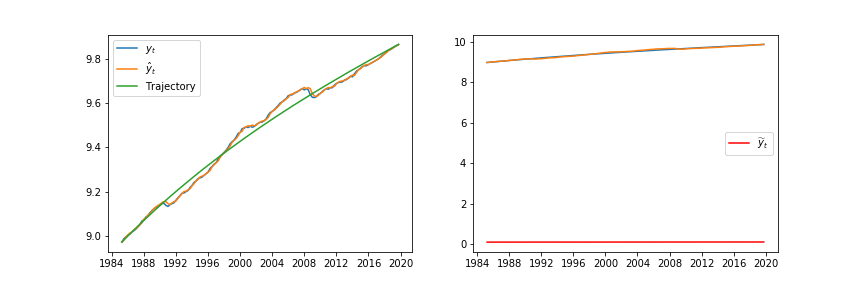
\includegraphics[width=\textwidth]{q1-fig}
\caption{}
\label{q1-fig}
\end{figure}
\end{proof}

\end{enumerate}

\begin{prob}
\textbf{Frequentist Asymptotics -- Part I}
\\ \\
Consider the AR(1) model 
\[
	y_t = \phi y_{t-1} + \eta_t, \qquad \eta_t \sim \text{iid N}(0, \sigma_\eta^2),
\]
where $|\phi| <1$.
\end{prob}

\begin{enumerate}
\item
What is the difference between a conditional and unconditional likelihood function?

\begin{proof}
Let $y = (y_1,\dotsc, y_T)'$, and $\theta = (\phi, \sigma_\eta^2)'$. The conditional likelihood function $p(y \mid y_0, \theta)$ 
assumes $y_0$ is known and conditions on this initial observation. The unconditional likelihood function $p(y, y_0 \mid \theta) = p(y \mid y_0, \theta) p (y_0 \mid \theta)$ is the joint density of the entire sample and therefore contains more ``information''.
\par
The first-order Markovian structure and iid Gaussian innovations of the AR(1) yields a conditional likelihood function of the factorized form
\begin{align*}
	p(y \mid y_0, \theta) &= \prod_{t=1}^T p(y^t \mid y^{t-1}, y_0, \theta) 
	= \frac{1}{(2 \pi \sigma_\eta^2)^{T/2}} \exp\left(-\frac{1}{2 \sigma_\eta^2} \sum_{t=1}^T (y_t - \phi y_{t-1})^2 \right),
\end{align*}
where $y^{t_k}  = (y_1,\dotsc, y_{t_k})'$.
\par
To obtain the unconditional likelihood function, notice that if the process $\{y_t\}$ was initialized in the infinite past, then the assumption that $|\phi | <1$ implies that $y_0 \sim N(0, \sigma_\eta^2/(1-\phi))$,  and hence 
\[
	p(y, y_0 \mid \theta) = \frac{(1-\phi^2)^{1/2}}{(2 \pi \sigma_\eta^2)^{(T+1)/2}} \exp\left(-\frac{1}{2 \sigma_\eta^2}  \sum_{t=1}^T (y_t - \phi y_{t-1})^2 + \frac{(1-\phi^2)}{2 \sigma_\eta^2} y_0^2 \right)
\]
\end{proof}

\item 
Derive the conditional MLE of $\phi$, denoted $\hat \phi$. 

\begin{proof} 
The conditional log likelihood is
\[
	\log p(y \mid y_0, \theta) = -\frac{T}{2} \log 2 \pi - \frac{T}{2}  \log \sigma_\eta^2 - \frac{1}{2 \sigma_\eta^2} \sum_{t=1}^T(y_t- \phi y_{t-1})^2.
\]
To find the MLE of $\phi$  we only solve 
\[
	\min_{\phi} \sum_{t=1}^T (y_t- \phi y_{t-1})^2,
\]
since maximization of $p(y \mid y_0,\theta)$ with respect to $\phi$ only depends on this expression. The first order condition necessary condition for is 
\begin{align*}
	\sum_{t=1}^T (y_t- \phi y_{t-1})y_{t-1} = 0 \iff & \sum_{t=1}^T y_t y_{t-1} - \phi \sum_{t=1}^T  y_{t-1}^2  = 0 \\
	\iff & \sum_{t=1}^T y_t y_{t-1} = \phi \sum_{t=1}^T  y_{t-1}^2.
\end{align*}
Provided the variance of $y_{t-1}$ is nonzero, the MLE of $\phi$ is 
\[
	\hat \phi = \frac{\sum_{t=1}^T y_t y_{t-1}}{\sum_{t=1}^T y_{t-1}^2} 
	= \phi + \frac{T^{-1} \sum_{t=1}^T y_{t-1} \eta_t}{T^{-1} \sum_{t=1}^T y_{t-1}^2}. 
\]
\end{proof}


\item
Show that $\hat \phi$ is a consistent estimator of $\phi$.

\begin{proof}
If $\eta_t$ is strictly stationary and ergodic and $|\phi| <1$, then $y_t$, $y_t^2$, $y_ty_{t-1}$, and $y_{t-1} \eta_t$ are all measurable transformations of $\eta_t$. Then by the law of large numbers for strictly stationary and ergodic processes (White, 1984), the limit of the denominator is
\[
	\frac{1}{T}\sum_{t=1}^T y_{t-1}^2 \to \E y_{t-1}^2 = \frac{\sigma_\eta^2}{1-\phi^2}.
\] 
Now we derive the limit of the numerator. By independence, $y_{t-1} \eta_t$ is a martingale difference sequence, i.e., $\E y_{t-1} \eta_t = 0$ with second moment
\[
	\E y_{t-1}^2\eta_t^2 =\E y_{t-1}^2 \E \eta_t^2 =\frac{\sigma_\eta^2}{1-\phi^2} \sigma_\eta^2.
\]
So again by the law of large numbers for strictly stationary and ergodic processes 
\[
	\frac{1}{T}\sum_{t=1}^T y_{t-1}\eta_t \to \E y_{t-1}\eta_t = 0.
\]
Combining these results implies $\hat \phi - \phi \to 0$.
\end{proof}

\item
Derive the limiting distribution of $\hat\phi$.

\begin{proof}
By the central limit theorem for martingale difference sequences (White, 1984), 
\[
	\frac{1}{\sqrt T} \sum_{t=1}^T y_{t-1}\eta_t \Rightarrow N\left(0, \frac{\sigma_\eta^4}{1-\phi^2} \right)
\]
and therefore
\[
	\sqrt T(\hat \phi - \phi) \Rightarrow N(0, V),
\]
where $V = \sigma_\eta^4/(1-\phi^2) \cdot (\sigma_\eta^{2}/(1-\phi^2))^{-2} = 1-\phi^2$.
\end{proof}

\item
Suppose data is generated from an AR(2) model 
\begin{equation}\label{eq:4}
	y_t = \gamma_1 y_{t-1} + \gamma_2 y_{t-2} + \eps_t, \qquad \eps_t \sim \text{iid N}(0, \sigma_\eps^2),
\end{equation}
but the econometrician estimates the above AR(1) model. What are the probability limits of $\hat \phi$ and $\hat\sigma_\eta^2$ in terms of $(\gamma_1, \gamma_2, \sigma_\eps^2)$?

\begin{proof}
Assume that the coefficients $\gamma_1$ and $\gamma_2$ satisfy the stationarity conditions. By the law of large numbers for strictly stationary and ergodic processes, the denominator converges to 
\[
	\frac{1}{T} \sum_{t=1}^Ty_{t-1}^2 \to  \gamma(0) = \frac{1-\gamma_2}{(1 + \gamma_2)((1-\gamma_2)^2 - \gamma_1^2)}\sigma_\eps^2,
\]
and the numerator converges to
\[
	\frac{1}{T}\sum_{t=1}^T y_t y_{t-1} \to \gamma(1) = \frac{\gamma_1}{1-\gamma_2}\gamma(0).
\]
So 
\[
	\hat \phi \to \frac{\gamma_1}{1-\gamma_2}
\]
\par
To derive $\hat \sigma_\eta^2$, first differentiate the conditional log likelihood with respect to $\sigma_\eta^2$, which yields the first-order necessary condition
\[
	-\frac{T}{2\sigma_\eta^2} - \frac{1}{2 \sigma_\eta^4} \sum_{t=1}^T (y_t- \phi y_{t-1})^2 = 0,
\]
which gives
\begin{align*}
	\hat \sigma_\eta^2 &= \frac{1}{T}\sum_{t=1}^T (y_t- \hat \phi y_{t-1})^2  \\
	&= \frac{1}{T}\sum_{t=1}^T (y_t^2- 2\hat \phi y_t y_{t-1} + \hat \phi^2 y_{t-1})^2 \\
	&= \frac{1}{T}\sum_{t=1}^T y_t^2- 2\hat \phi \frac{1}{T}\sum_{t=1}^T y_t y_{t-1} + \hat \phi^2 \frac{1}{T}\sum_{t=1}^T y_{t-1}^2 \\
	&= \frac{1}{T} \sum_{t=1}^T y_t^2 - 2 \left(\frac{T^{-1} \sum_{t=1}^T y_t y_{t-1}}{T^{-1} \sum_{t=1}^T y_{t-1}^2}\right)  \frac{1}{T}\sum_{t=1}^T y_t y_{t-1} + \left( \frac{T^{-1} \sum_{t=1}^T y_t y_{t-1}}{T^{-1} \sum_{t=1}^T y_{t-1}^2} \right)^2 \frac{1}{T}\sum_{t=1}^T y_{t-1}^2 \\
	&= \frac{1}{T} \sum_{t=1}^T y_t^2 - \frac{(T^{-1} \sum_{t=1}^T y_t y_{t-1})^2}{T^{-1} \sum_{t=1}^T y_{t-1}^2}. 
\end{align*}	
By the law of large numbers,
\[
	\frac{1}{T} \sum_{t=1}^T y_t^2 \to \E y_t^2 = \gamma(0)
\]
and
\[
	\frac{1}{T} \sum_{t=1}^T y_{t-1}^2 \to \gamma(0),
\]
and, by the continuous mapping theorem and law of large numbers,
\[
	\left(\frac{1}{T}\sum_{t=1}^T y_t y_{t-1} \right)^2 \to (\E y_ty_{t-1})^2 
	= \gamma(0)^2 \left(\frac{\gamma_1}{1 - \gamma_2}\right)^2.
\]
Hence
\[
	\hat \sigma_\eta^2 \to \gamma(0) -  \left(\frac{\gamma_1}{1 - \gamma_2}\right)^2\gamma(0) 
	= \frac{\sigma_\eps^2}{1-\gamma_2^2}, 
\]
since
\begin{align*}
	\gamma(0) -  \left(\frac{\gamma_1}{1 - \gamma_2}\right)^2\gamma(0) 
	&= \gamma(0) \left(1-\frac{\gamma_1^2}{(1 - \gamma_2)^2}\right) \\
	&= \frac{(1-\gamma_2)\sigma_\eps^2}{(1 + \gamma_2)((1-\gamma_2)^2 - \gamma_1^2)} \frac{(1-\gamma_2)^2- \gamma_1^2}{(1-\gamma_2)^2}  
	= \frac{\sigma_\eps^2}{1-\gamma_2^2}.
\end{align*}
\end{proof}
\end{enumerate}


\begin{prob}
\textbf{Bayesian Analysis -- Part II} 
\\ \\
Consider the AR(1) model 
\[
	y_t = \phi y_{t-1} + \eta_t, \qquad \eta_t \sim \text{iid N} (0, \sigma_\eta^2).
\]
\end{prob}


\begin{enumerate}
\item
Consider the following prior for $\phi$: $\phi \sim N(0, \tau^2)$. Show that the posterior distribution of $\phi$ is normal and derive its mean and its variance.

\begin{proof}
Combining the likelihood function with prior distribution gives the posterior distribution:
\begin{align*}
	p(\phi \mid y) & \propto p(y \mid \phi) p(\phi) \\ 
	& \propto \exp\left\{- \frac{1}{2} \left( \sum_{t=1}^{T} (y_t - \phi y_{t-1} )^2  +\frac{\phi^2}{\tau^2} \right) \right\} \\
	&\propto \exp\left\{- \frac{1}{2}  \left( \sum_{t=1}^{T} y_t^2 - 2 \phi \sum_{t=1}^{T} y_t y_{t-1} + \phi^2 \left(\sum_{t=1}^{T} y_{t-1}^2 + \tau^{-2} \right) \right)\right\} \\
	& \propto \exp\left\{ - \frac{1}{2}\frac{\phi^2 - 2 \phi \sum_{t=1}^{T} y_t  y_{t-1} (\sum_{t=1}^{T}y_{t-1}^2 + \tau^{-2})^{-1}}{(\sum_{t=1}^{T} y_{t-1}^2 + \tau^{-2})^{-1}} \right\} \\
	& \propto \exp\left\{ - \frac{1}{2}\frac{(\phi - \sum_{t=1}^{T} y_t y_{t-1} (\sum_{t=1}^{T} y_{t-1}^2 + \tau^{-2})^{-1})^2}{(\sum_{t=1}^{T}  y_{t-1}^2 + \tau^{-2})^{-1}} \right\},
\end{align*}
which is of the form of a normal distribution: 
\[
	\phi \mid y\sim N(\bar \phi, \overline V),
\]
where 
\begin{align*}
	\bar \phi &=\frac{ \sum_{t=1}^{T} y_t y_{t-1}}{\sum_{t=1}^{T}y_{t-1}^2 + \tau^{-2}} \\
	\overline V &= \left(\sum_{t=1}^{T} y_{t-1}^2 + \tau^{-2} \right)^{-1}.
\end{align*}
\end{proof}


\item
What happens to the posterior distribution if you let $\tau$ go to zero or infinity?
 
\begin{proof}
Letting the prior standard deviation go to zero $\tau \to 0$, 
\[
	\bar \phi =\frac{\tau^2 \sum_{t=1}^{T} y_t y_{t-1}}{\tau^2 \sum_{t=1}^{T}y_{t-1}^2 + 1} \to 0,
\]
and 
\[
	\overline V = \frac{\tau^2}{\sum_{t=1}^{T} y_{t-1}^2 + 1} \to 0,
\]
meaning that the posterior mean and variance converge to their prior mean and variance. 
\par
Letting $\tau \to \infty$, 
\[
	\bar \phi \to \frac{\sum_{t=1}^T y_t y_{t-1}}{\sum_{t=1}^T y_{t-1}^2} 
	= \hat \phi,
\]
and 
\[
	\overline V \to  \left(\sum_{t=1}^{T} y_{t-1}^2 \right)^{-1}.
\]
\end{proof}


\item
Suppose the goal is to forecast $y_{T+2}$ based on information up until time
$T$, given by the sample $y = (y_1,\dotsc,y_T)'$. Show that under the loss function
\begin{equation}
	L(y_{T+2}, \hat y_{T+2 \mid T}) = (y_{T+2} - \hat y_{T+2 \mid T})^2,
\end{equation}
where $y_{T+2}$ is the actual value and $\hat y_{T+2 \mid T}$ is the predicted value, the optimal (minimizing posterior expected loss) forecast is given by
\begin{equation}
	\hat y_{T+2\mid T}^* = \E(y_{T+2} \mid y) = \E_y y_{T+2}
\end{equation}

\begin{proof}
To verify this claim, consider basing $\hat y_{T+2\mid T}^*$ on any function $g$ not equal to $\E_y y_{T+2}$. Under $g$, adding and subtracting the conditional expectation, the expected posterior loss is
\begin{align*}
	& \E_y (y_{T+2} - g(y))^2 \\
	&= \E_y (y_{T+2} - \E_y y_{T+2}  + \E_y y_{T+2} - g(y))^2  \\
	&= \E_y (y_{T+2} - \E_y y_{T+2})^2 + 2 \E_y ((y_{T+2} - \E_y y_{T+2}) \E_y (y_{T+2}  - g(y)) + \E_y \E_y (y_{T+2} - g(y))^2
\end{align*}
If we condition on $y_{T+2\mid T}$ in the cross product term and take expectations, then
\begin{align*}
	& \E_y (y_{T+2} - \E_y (y_{T+2} \mid y_{T+2 | T})) \E_y ((y_{T+2} \mid y_{T+2 | T}) - g(y)) \mid y_{T+2 | T}) \\
	&= \E_y ((y_{T+2} \mid y_{T+2 \mid T}) - g(y)) \E_y (y_{T+2} - \E_y (y_{T+2} \mid y_{T+2 | T})) \\
	&=\E_y ((y_{t+2} \mid y_{T+2 | T}) - g(y)) \cdot 0 = 0,
\end{align*}
where the last equality follows from the law of iterated projections. Our expected quadratic loss is now 
\[
	\E_y (y_{T+2} - g(y))^2 = \E_y (y_{T+2} -  \E_y y_{T+2} )^2 + \E_y (y_{T+2} - g(y))^2,
\]
which attains a minimum when $g$ is such that $g(y) = \E_y y_{T+2}$.
\end{proof}

\item
Using the results from (i), calculate the optimal two-step ahead predictor
for the estimated AR(1) model.

\begin{proof}
Since $\eta_\tau$ for $\tau >  T$ is independent of $\phi \mid y$, we have 
\begin{align*}
	\hat y_{T+2| T}^* &= \E_y (\phi^2y_T + \phi \eta_T + \eta_{T+1}) \\
	&=y_T \E_y\phi^2  + \E_y \phi \E_y \eta_T + \E_y \eta_{T+1} \\
	&= (\overline V + \phi^2) y_T.
\end{align*}
\end{proof}
\end{enumerate}


\end{document}
